\documentclass[border=6pt]{standalone}
\usepackage{tikz}
\usetikzlibrary{arrows.meta}
\begin{document}
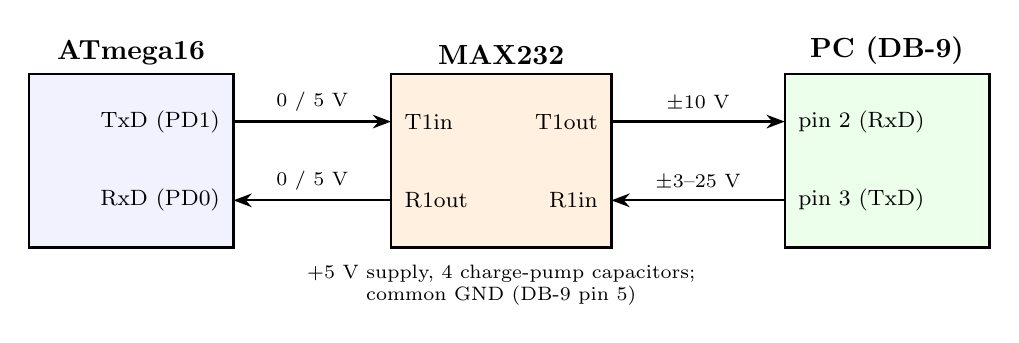
\begin{tikzpicture}[>=Stealth,font=\small]
\draw[thick,fill=blue!5] (0,0) rectangle (2.6,-2.2); \node[font=\bfseries,anchor=south] at (1.3,0) {ATmega16};
\draw[thick,fill=orange!12] (4.6,0) rectangle (7.4,-2.2); \node[font=\bfseries,anchor=south] at (6.0,0) {MAX232};
\draw[thick,fill=green!8] (9.6,0) rectangle (12.2,-2.2); \node[font=\bfseries,anchor=south] at (10.9,0) {PC (DB-9)};
\node[font=\footnotesize,anchor=east] at (2.55,-0.6) {TxD (PD1)};
\node[font=\footnotesize,anchor=east] at (2.55,-1.6) {RxD (PD0)};
\node[font=\footnotesize,anchor=west] at (4.65,-0.6) {T1in}; \node[font=\footnotesize,anchor=east] at (7.35,-0.6) {T1out};
\node[font=\footnotesize,anchor=west] at (4.65,-1.6) {R1out}; \node[font=\footnotesize,anchor=east] at (7.35,-1.6) {R1in};
\node[font=\footnotesize,anchor=west] at (9.65,-0.6) {pin 2 (RxD)};
\node[font=\footnotesize,anchor=west] at (9.65,-1.6) {pin 3 (TxD)};
\draw[->,thick] (2.6,-0.6) -- (4.6,-0.6) node[midway,above,font=\scriptsize]{0 / 5 V};
\draw[<-,thick] (2.6,-1.6) -- (4.6,-1.6) node[midway,above,font=\scriptsize]{0 / 5 V};
\draw[->,thick] (7.4,-0.6) -- (9.6,-0.6) node[midway,above,font=\scriptsize]{$\pm$10 V};
\draw[<-,thick] (7.4,-1.6) -- (9.6,-1.6) node[midway,above,font=\scriptsize]{$\pm$3--25 V};
\node[font=\scriptsize,align=center,anchor=north] at (6.0,-2.3) {+5 V supply, 4 charge-pump capacitors;\\common GND (DB-9 pin 5)};
\end{tikzpicture}
\end{document}
